\newcommand{\orgmode}{\texttt{org-mode}}
\newcommand{\Makefile}{\mintinline{shell}{Makefile}}
\newcommand{\context}{\mintinline{shell}{context}}
\newcommand{\CC}{C\nolinebreak\hspace{-.05em}\raisebox{.4ex}{\tiny\bf +}\nolinebreak\hspace{-.10em}\raisebox{.4ex}{\tiny\bf +}}
\def\CC{{C\nolinebreak[4]\hspace{-.05em}\raisebox{.4ex}{\tiny\bf ++}}}
\newcommand{\qmcchem}{\textsc{QMC=Chem}}
\newcommand{\champ}{\textsc{Champ}}
\newcommand{\turbo}{\textsc{TurboRVB}}
\newcommand{\QMCkl}{\textsc{\ac{QMCkl}}}

\section{Introduction}

There are three different \ac{QMC} codes in the \ac{TREX} \ac{CoE},
\turbo{}, \champ{}, and \qmcchem{}, each with its own strengths and
weaknesses. Instead of optimizing the three codes independently for
exascale architectures, or re-writing a new monolithic code, our
strategy is instead to design a new library, \QMCkl{}, containing
the best of each code. The functions available in this library will
allow all three codes to benefit from the optimal implementation of
the major kernels of \ac{QMC}.
%We believe that this library will be
%adopted by the community beyond the \ac{TREX} \ac{CoE}.
The three main objectives driving the development of \QMCkl{} are
\emph{performance}, \emph{productivity} and \emph{portability}.

\subsection{Performance}

The ultimate goal of \QMCkl{} is to provide a high-performance
implementation of the main computational kernels involved in \ac{QMC}
methods, well adapted to exascale machines.
In this particular \ac{WP}, we focus on the
definition of the \ac{API}, the tests, and on a \emph{pedagogical}
presentation of the algorithms. The high-performance aspects are
delegated to \ac{WP}3, but there is nevertheless a strong interaction
between these two \acp{WP} because the design of the data structures
and the \ac{API} are guided by the possibility to enable a
high-performance implementation of the computational kernels.
For instance, the data structures should be such that the memory
access patterns are efficient both on CPUs and accelerators, and the
library should not be too restrictive on how the memory is allocated
to give enough freedom to the developers of the \ac{HPC} variants to
allocate memory on the CPU or \ac{GPU}, pinned or not, etc.

The main objective of this pedagogical implementation of the library
is to provide a reference implementation of the kernels such that
\ac{HPC} experts involved in \ac{WP}3 will be able to use it to rewrite
optimized versions of the functions described in this library, using the same
\ac{API}.

\subsection{Portability}

\QMCkl{} should take advantage of exascale machines. In terms of hardware,
many different architectural designs are proposed for exascale
supercomputers. Some are CPU-based, others are \ac{GPU}-based, multiple vendors
propose different CPUs (Intel, AMD, ARM,~\dots) or \acp{GPU} (Intel,
NVidia, AMD,~\dots). In this context, we have to propose a library that
will take advantage of any of these combinations so we can't rely on 
a vendor-specific software stack like Intel's \ac{MKL} or Nvidia's
Cuda language. Instead, we
will rely on free software and open standards such as OpenMP, but the BSD
licence we have adopted also gives the freedom to the community to
modify \QMCkl{} and propose vendor-specific implementations of \QMCkl{}.

For maximum portability, we have chosen to propose an \ac{API} compatible with
the C language. In this way, we guarantee that \QMCkl{} will be usable in
\emph{all} the QMC codes used by the \ac{QMC} community, although these codes
are written in different programming languages (C, C++, Python, Fortran, etc.).

\subsection{Productivity}

\ac{QMC} methods are still under heavy development. Therefore,
scientists need to be able to understand the code to modify the
algorithms and propose new methods. It is not realistic to believe
that any physicist/chemist will be able to read and develop a highly optimized
C++ code tuned by \ac{HPC} experts. Similarly, it is not realistic
either to believe that a code written by a random physicist/chemist will
be easily ported to \ac{GPU} by a \ac{HPC} expert without requiring a deep
restructuring of the code. If a compromise
is chosen between these two extremes, it is likely that it will
converge to a code difficult to maintain by the physicist and
difficult to optimize by the \ac{HPC} expert. Therefore our choice is to
develop at least two libraries with the same \ac{API}: first a
\emph{pedagogical} implementation (the objective of the current \ac{WP})
designed for physicists/chemists, and then multiple high-performance
implementations of this library.


\section{Development environment}

\subsection{Literate programming}

As the focus of this pedagogical implementation of \QMCkl{} is documentation,
we use literate programming using {\orgmode} files.\cite{schulte_2012,orgmode}
Hence, the code and the documentation are produced with the same
source files, allowing the programmers to write \LaTeX{} formulas and
use tables or figures together with the corresponding code in the same
files.
This method has proven to be particularly efficient in maintaining the
documentation consistent with the source code, and literate
programming is now becoming a very popular technique thanks to the
development of Jupyter notebooks.
Here, we have chosen {\orgmode} as it allows the simultaneous usage of
multiple languages in the same notebook, and also doesn't impose to
use a web browser for editing.

\subsection{Configuration}

In the first months, a large effort was put in preparing the
foundations of the library: the coding standards and rules, GNU Autotools
configuration scripts, Makefiles, scripts to generate automatically
the code and the documentation, unit testing, continuous integration,
etc. It is important not to neglect the importance of all these
developments which are not directly visible from outside of the project.
Having spent a large effort of preparation pays a lot in the long term
since is can dramatically enhance the productivity of the contributors
of the library.
Now that this effort has been done, we are in a position where we are highly
productive in implementing new kernels.

\subsection{Control of Numerical accuracy}

An original feature of \QMCkl{} is that the numerical precision of the
implemented kernels will be monitored during the whole development
process of the library.
With this aim in mind, the \ac{UVSQ} team has proposed an internship
to a master's student, Aurélien Delval, to build a continuous
integration system which, instead of monitoring if tests pass or fail,
keeps track of the numerical accuracy of the implemented kernels of \QMCkl{}.

This tools relies on Verificarlo,\cite{verificarlo} a software
developed by TREX members that implements Monte Carlo arithmetic at
the binary level via the LLVM compiler. The continuous integration
tool Verificarlo-CI has been integrated into GitHub actions, such that
by inserting probes in the tests provided with \QMCkl{} the numerical
accuracy can be monitored each time a new version of the code is
pushed on the server.

\begin{figure}
\centering
  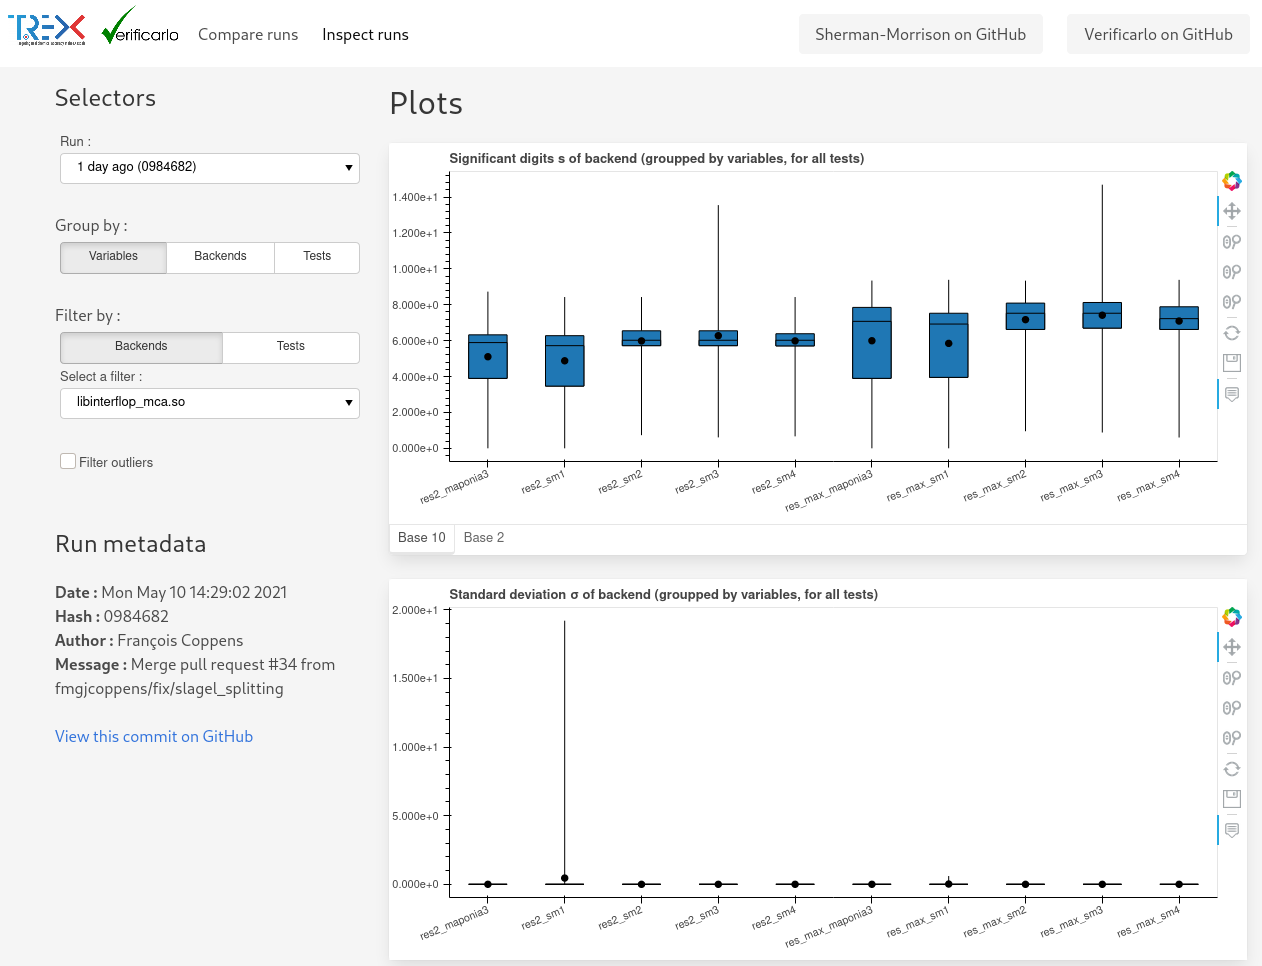
\includegraphics[width=0.9\textwidth]{images/inspect_runs.png}
  \caption{Verificarlo-CI: graphical display of the precision obtained
    with multiple kernels.}
    \label{fig:vfci}
\end{figure}
A nice graphical interface is proposed to compare the accuracy
obtained with different versions, or to display the fluctuation of
the results obtained by different kernels (Fig.~\ref{fig:vfci}).
A tutorial about how to use Verificarlo-CI is presented in appendix.

\subsection{Introduction of TREXIO in QMCkl}

The input of a \ac{QMC} calculation is a wave function, which
contains usually a large number of parameters of different nature:
nuclear coordinates, atomic basis set parameters, pseudo-potential
parameters, molecular orbital coefficients, Slater determinant
expansion coefficients, etc.
Hence, initializing \QMCkl{} can quickly become cumbersome to the users
of the library.

\ac{TREXIO} is the file format and input/output library developed in
\ac{WP}2. It allows to store all the information relative to a wave
function in a file, and provides functions to retrieve easily all
these parameters. 

To simplify the initialization procedure of the library, we have
introduced the possibility to load, with a single function call, all the
wave function parameters contained in a \ac{TREXIO} file. This simple
change is extremely beneficial to the user experience.


\section{Implemented kernels}

The documentation of the current status of the library is available
at \url{https://trex-coe.github.io/qmckl}, and the source code is
available on the GitHub repository at \url{https://github.com/trex-coe/qmckl}.
In the last few months, the majority of the effort was put in
implementing and documenting kernels.  Our objective for this milestone
was to provide a library that is capable of computing the local energy
(the central quantity in \ac{QMC}) for any arbitrary system described
by a Slater determinant using a Gaussian atomic basis set:
\newcommand{\eloc}{E_{\text{loc}}}
\newcommand{\rr}{\mathbf{r_1^\uparrow,\dots,r_M^\uparrow, r_{M+1}^\downarrow,\dots,r_N^\downarrow}}
\[
\eloc\left(\rr\right) = \frac{\hat{T}{\Psi\left(\rr\right)}}{\Psi\left(\rr\right)}
+ V\left(\rr\right)
\]
with
\[
\Psi\left(\mathbf{r_1^\uparrow,\dots,r_M^\uparrow, r_{M+1}^\downarrow,\dots,r_N^\downarrow}\right) = 
\left|
\begin{array}{ccc}
\phi_1\left(\mathbf{r}_1^\uparrow\right) & \cdots & \phi_1\left(\mathbf{r}_M^\uparrow\right) \\
\vdots & \ddots & \vdots \\
\phi_M\left(\mathbf{r}_1^\uparrow\right) & \cdots & \phi_M\left(\mathbf{r}_M^\uparrow\right) 
\end{array}
\right|
\left|
\begin{array}{ccc}
\phi_{M+1}\left(\mathbf{r}_{M+1}^\downarrow\right) & \cdots & \phi_{M+1}\left(\mathbf{r}_N^\downarrow\right) \\
\vdots & \ddots & \vdots \\
\phi_N\left(\mathbf{r}_{M+1}^\downarrow\right) & \cdots & \phi_N\left(\mathbf{r}_N^\downarrow\right) 
\end{array}
\right|
\]

We have reached successfully this stage, and the implemented kernels are
described in this section.

The electron-electron $V_{\text{ee}}$ and nucleus-nucleus $V_{\text{NN}}$
repulsion contributions to the potential, as well as the electron-nucleus
$V_{\text{eN}}$ attraction have been implemented. These kernels are relatively
straightforward. However, the computation of the kinetic energy $\hat{T}$ is
more complex since it requires the evaluation of the wave function at the
electron positions and its second derivative. In this section, we give some
information about the kernels implemented for the computation of the kinetic
energy.

\subsection{Native linear algebra functions}

One of the main development guidelines is to maximize the use
of \ac{BLAS}-like operations in the main kernels. The main \ac{BLAS} operations are
as follows:

\begin{itemize}
\item Level 1 - Operations (e.g. scalar product) on two vectors.
\item Level 2 - Operations involving Matrix and vector (e.g. Matrix vector product).
\item Level 3 - Operations involving two matrices (Matrix times Matrix).
\end{itemize}

Incorporating these basic operations in developing the main algorithms is key to
achieve an optimal implementation of the library. However, the efficiency of these key \ac{BLAS}
functions depend on the type of hardware (i.e. CPU, or accelerator) and require a
tailored approach. Therefore, in \QMCkl{}, we have chosen to abstract the
calls to such libraries with standard \QMCkl{} functions such as
\mintinline{C}{qmckl_dgemm} and \mintinline{C}{qmckl_invert} for matrix
multiplication and inversion. This has a two-fold advantage of standardizing
the \ac{API} and enabling hardware specific optimizations by \ac{HPC} experts
without breaking user-space.

A second and significant advantage of providing native implementations of
such key functions is to enable new developers and scientists to easily
setup and install a minimal version of \QMCkl{} without struggling with
a large set of dependencies, thus enabling easy access to new users.

\subsection{Atomic basis functions}

The atomic basis set is defined as a list of shells. Each shell $s$ is
centered on a nucleus $A$, possesses a given angular momentum $l$ and a
radial function $R_s$. The radial function is a linear combination of
\emph{primitive} functions that can be of type Slater ($p=1$)  or
Gaussian ($p=2$):
\[
  R_s(\mathbf{r}) = \mathcal{N}_s |\mathbf{r}-\mathbf{R}_A|^{n_s}
  \sum_{k=1}^{N_{\text{prim}}} a_{ks}\, f_{ks}
 \exp \left( - \gamma_{ks} | \mathbf{r}-\mathbf{R}_A | ^p \right).
\]

In the case of Gaussian functions, $n_s$ is always zero.  The
normalization factor $\mathcal{N}_s$ ensures that all the functions of
the shell are normalized (integrate to unity). Usually, basis sets are
given a combination of normalized primitives, so the normalization
coefficients of the primitives, $f_{ks}$, need also to be provided.

\acp{AO} are defined as
\[
\chi_i (\mathbf{r}) = \mathcal{M}_i\, P_{\eta(i)}(\mathbf{r})\, R_{\theta(i)} (\mathbf{r})
\] 
where $\theta(i)$ returns the shell on which the \ac{AO} is expanded, and
$\eta(i)$ denotes which angular function is chosen and $P$ are the
generating functions of the given angular momentum $\eta(i)$.  Here,
the parameter $\mathcal{M}_i$ is an extra parameter which allows the
normalization of the different functions of the same shell to be
different, as in GAMESS for example.


\subsection{Molecular orbitals}

The calculation of molecular orbitals (MOs) is one such key kernel which can
become a bottleneck unless one uses a highly optimized implementation.
In this documentation implementation, we have provided an extremely simple
algorithm which uses a \ac{BLAS} Level 3 call to a matrix multiplication
routine (\mintinline{C}{qmckl_dgemm}),
\[
  \phi_i(r) = \sum_{j}C_{i,j}\chi_j(r),
    \label{eq:mos}
\]
thus enabling \ac{HPC} experts to easily identify and optimize the calculation
of molecular orbitals. Note that in this pedagogical implementation of the
library, the calculation of the \acp{MO} uses a native call to the
\mintinline{C}{qmckl_dgemm} function.

\subsection{Slater Determinants}

Once the molecular orbitals are implemented, the Slater matrix $S_{ij} = \phi_i(\mathbf{r}_j)$,
where $\mathbf{r}_j$ represents the Cartesian coordinates of the $j$-th electron, needs to be
calculated along with its inverse $S^{-1}$.
  
Here again we encounter a general  function
\mintinline{C}{qmckl_invert} for which we have also provided a small native
library. An efficient implementation of the inverse is key since the 
scaling of the algorithm is cubic. We have specially provided hand-coded functions for
the calculation of the inverse of small matrices ($M\le 5$) for which the
$\mathcal{O}(N!)$ algorithm is faster than calling external library functions.
Efficient methods based on the adjoint of a matrix \cite{MCMQC} are used to
compute the gradient of the Slater matrix, which is necessary for the 
computation of the drift vector used in the dynamics of the
electrons, and the Laplacian of the Slater matrix required for the computation of
the electronic kinetic energy. Both quantities involve the computation of
the inverse of the Slater matrix.

For single determinant wave functions, computing the inverse of the Slater
matrix translates to a call to \mintinline{C}{qmckl_invert} function. For
multi-determinant wave functions, more sophisticated kernels need to be
implemented as presented in the next subsection.

For the computation of the gradient and Laplacian, a special function
\mintinline{C}{qmckl_dgemm_diag} has been implemented and used which provides
the diagonal of the result of a matrix product. 

\subsection{Inverse of the Slater matrix}

The Sherman-Morrison formula computes the inverse of the sum of a
non-singular matrix $A$ of size $n \times n$ and an outer product
$uv^T$ of vectors $u$ and $v$ of size $n$ :

\begin{equation}
    (A + uv^T) = A^{-1} - \frac{A^{-1} uv^T A^{-1}}{1 + v^T A^{-1} u}
    \label{eq:sherman}
\end{equation}

This formula is especially useful when one is interested in the
inverse of $A + uv^T$ and $A^{-1}$ is already available. Thus, this 
method only requires to apply a small number of rank-1 updates $A + u_i v_i^T$
to a matrix, and is computationally cheaper than inverting the matrix
with standard techniques like LU-decomposition.

This algorithm is the main bottleneck of multi-determinant
calculations, so it is crucial to have the most efficient
implementation. In addition, this algorithm is known to be responsible
for propagating numerical errors, so a careful study of the
performance and of the accuracy of multiple kernels was realized,
thanks to Verificarlo-CI. The involved algorithms are:
\begin{center}
\begin{tabular}{ll}
  SM1:      & The simple Sherman-Morrison formula (Eq.~\eqref{eq:sherman}) \\
  SM2:      & Slagel's splitting method\cite{slagel_splitting} \\
  SM3:      & Reordering of the updates \\
  SM4:      & Reordering of the updates, then Slagel's splitting \\
  MaponiA3: & Maponi's pivoting technique\cite{maponi} \\
\end{tabular}
\end{center}



\section{Applications of QMCkl}

The proposed library can already be used in production and for
methodological developments. A few examples are presented in this section.

\subsection{Jastrow factor in QMC=Chem}

The strength of \qmcchem{} is large multi-determinant expansions, so very
little effort was put in the development of the Jastrow factor. Only the
simplest form of Jastrow factor was initially available. As shown above, the
sophisticated form of Jastrow factor developed in \champ{} was introduced
in \QMCkl{}, so this functionality has been made quickly available
in \qmcchem{} by calling the \QMCkl{} appropriate functions.

\subsection{Sherman-Morrison-Woodbury kernels in QMC=Chem}

The Sherman-Morrison-Woodbury formula is the most important kernel in
simulations involving large multi-determinant expansions. Hence, it has
been carefully optimized in \qmcchem{} in the past. The kernels
developed in \QMCkl{} can now be called in \qmcchem{} in order
to compare the performance of the library with \qmcchem{}. The
comparisons are still ongoing, but is now easy to measure the
efficiency of the kernels developed in \QMCkl{} since we can now
measure their efficiency beyond benchmark situations, under real
simulation conditions.

\subsection{Exploratory methods using neural networks}

In \ac{WP}4, one project consists in using a neural network as a
form of Jastrow factor. Many frameworks for machine learning are in
Python or Java, which can't be easily used inside a Fortran program.
Moreover, for this particular project we need to evaluate the gradient
and Laplacian of the Jastrow factor, which requires the ability to
compute derivatives of the neural network. Computing derivatives is
particularly easy with the PyTorch package which is for the Python
programming language. In this project, we will use Python as the main
language, PyTorch for the neural network and \QMCkl{} for the
Slater-determinant component. This project will illustrate the
versatility of \QMCkl{}, and the importance of providing a library that
can be easily used in any programming language.


\subsection{Exascale-related algorithms}

Another project of \ac{WP}4 is the development of a novel algorithm
for \ac{DMC}, enabling an efficient load-balancing by
making the walkers de-synchronized. In this particular work, it is only
necessary to have a ``black box'' that computes the local energy and
the gradient of the wave function, which can be both provided by \QMCkl{}.
This work will first be realized in the Julia or in the Python
language, which are very good for quick prototyping. Then, once the
algorithm is validated on a large scale, it will be implemented in the
flagship codes.


\subsection{Debugging TREXIO files}

We expect the \ac{TREXIO} library to be widely adopted by the community of
quantum chemistry. But writing files in \ac{TREXIO} format requires the developer
to be well aware of the conventions used in the code, namely the normalization factors
of the basis functions, the order in which the Cartesian functions appear, etc.
It is important to provide a tool with \ac{TREXIO}, that will allow the developer to
check that the file written is valid. A good check is to very numerically that the
molecular orbitals are orthonormal. Passing this test implies that the data
relative to the basis set is consistent with the coefficients of the molecular
orbitals, so the \ac{TREXIO} file is valid. We have developed such a tool 
writing a simple program which calls \QMCkl{} to evaluate the molecular orbitals
at grid points.

\section{Future work}

\subsection{Development}

We have now reached a milestone where we are able to compute the local energy of an
arbitrary system described as a single determinant with a Gaussian basis set.
Reaching this stage enables the development of \ac{HPC} variants of the library in
\ac{WP}3, and the exploratory benchmarks to monitor the performance of the kernels on
CPUs and \acp{GPU} as well as the efficiency in the way they are scheduled.
However, there is still a lot of work to do in this \ac{WP} to make \QMCkl{}
usable by external developers.

The most important kernels that still need to be implemented are:
\begin{itemize}
  \item Kernels related to \acp{ECP}
  \item Multi-determinant wave functions
  \item Different forms of Jastrow factors
  \item Atomic basis functions input as values on grid points, to enable the use of
        arbitrary forms of atomic orbitals
  \item Cusp-fitting of the molecular orbitals at the nuclear positions
  \item Kernels related to periodic calculations
\end{itemize}

\subsection{Applications}

\newcommand{\qp}{\textsc{Quantum Package}}

We plan in the future to finish the integration of \QMCkl{} into the \ac{QMC}
codes of the \ac{CoE}. The efficient evaluation of the molecular orbitals is
now a performance bottleneck in \turbo{} that will be solved by using the
\ac{HPC} implementations of \QMCkl{}. Similarly, the three-body component of
the Jastrow factor in \champ{} will be accelerated by using \QMCkl{}.

Other applications of the library are possible beyond \ac{QMC}. For instance, 
the \qp{} code allows to combine \ac{DFT} with wave function
methods. \ac{DFT} methods require the computation of the one-electron density on 
a grid since many important integrals can only be approximated numerically. We
plan to use \QMCkl{} in \qp{} to accelerate the computation of the density grids
to demonstrate the potential of the library beyond \ac{QMC} simulations.


\clearpage


